
\chapter{A Second Order System; Shallow Water Waves}\pageoriginale\label{chap4}  

THE EXTENSION OF the ideas presented so far to higher order systems can be adequately explained on a typical example. We shall use the so called shallow water wave theory for this purpose, although the pioneering work was originally done in gas dynamics.

\section{The equations of shallow water theory}\label{chap4:sec4.1}

In shallow water theory the height $h(x,t)$ of the water surface above the bottom is small relative to the typical wave lengths; it is called shallow water theory or long wave theory depending on which aspects one wants to stress.

We take the bottom to be horizontal and neglect friction. Let the density of the water be normalized to unity and let the width be one unit.

Let $u(x,t)$ be the velocity, $p_0$ the atmospheric pressure and $(p_0+p'(x,t))$ the pressure in the fluid. In every section $x_2\leqq x\leqq x_1$ the mass is conserved, \ie
$$
\frac{d}{dt}\int\limits_{x_2}^{x_1}h(x,t)\,dx +q_1-q_2=0,
$$
where the flow $q=uh$.
\begin{figure}[H]
\centering
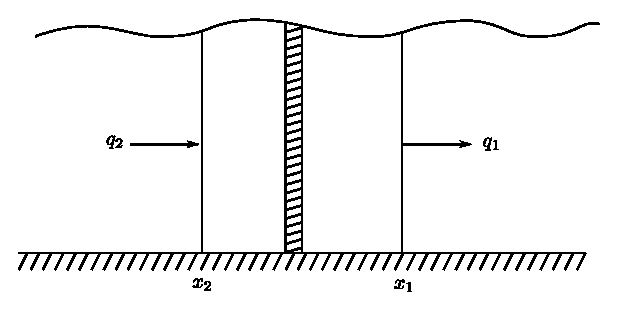
\includegraphics{figures/fig61-4.1.eps}
\caption{}
\label{chap1:fig4.1}
\end{figure}\pageoriginale

Taking the limit $x_2\to x_1$, we obtain 
\begin{align}
h_t & + q_x=0,\notag\\
\text{\ie} \qquad h_t & + (uh)_x=0\tag{4.1}\label{chap4:eq4.1}
\end{align}

This time a second relation between $u$ and $h$ is obtained from the conservation of the momentum in the $x$-direction. If we consider a section $x_2\leqq x\leqq x_1$, as shown in figure 4.1, a constant pressure $p_0$ acting all around the boundary, including free surface and bottom, is self-equilibrating. Therefore, only the excess pressure $p'$ contributes to the momentum balance. If $P(x,t)$ denotes the total excess pressure,
$$
P=\int\limits_0^h p'\,dy
$$
acting across a vertical section, the momentum equation is then
\begin{equation}
\frac{d}{dt}\int\limits_{x_2}^{x_1}\,hu \, dx =hu^2\mid_{x=x_2}-hu^2 \mid_{x=x_1} +P_2-P_1\tag{4.2}\label{chap4:eq4.2}
\end{equation}
where $P_i=P\left(x_i,t\right), i=1,2$.

The term in the left hand side of \eqref{chap4:eq4.2} is the total rate of change of momentum in the section $x_2\leqq x\leqq x_1$, and $hu^2\mid_{x=x_i}$, on the right,\pageoriginale denotes the momentum transport across the surface through $x=x_i(i=1,2)$. 

The basic assumption is shallow water theory is that the pressure is hydrostatic, \ie
\begin{equation}
\frac{\partial p}{\partial y}=-g\tag{4.3}\label{chap4:eq4.3}
\end{equation}
where $g$ is the acceleration due to gravity.

Integrating \eqref{chap4:eq4.3} and assuming the condition $p=p_0$ at the top $y=h$, we obtain
$$
p=p_0+g(h-y).
$$

Hence the total excess pressure is 
\begin{equation}
P=\int\limits_0^hg(h-y)\,dy =\frac{1}{2}\,gh^2\tag{4.4}\label{chap4:eq4.4}
\end{equation}
Equations \eqref{chap4:eq4.2} and \eqref{chap4:eq4.4} yield
\begin{equation}
\frac{d}{dt}\int\limits_{x_2}^{x_1}\,hu\,dx +\left[hu^2+\frac{1}{2}\,gh^2 \right]_{x_2}^{x_1}=0\tag{4.5}\label{chap4:eq4.5}
\end{equation}

The conservation form should be noted.

In the case of river flow discussed earlier, there would also be further terms on the right hand side of \eqref{chap4:eq4.5} due to the slope effect and friction; the slope is now omitted and frictional effects are neglected.

In the limit $x_2\to x_1$, \eqref{chap4:eq4.5} becomes 
\begin{equation}
(hu)_t+\left(hu^2+\frac{1}{2}\,gh^2\right)_x=0\tag{4.6}\label{chap4:eq4.6}
\end{equation}
Equations \eqref{chap4:eq4.1} and \eqref{chap4:eq4.6} provide the system for the determination of $u$ and $h$.

If\pageoriginale $h$ and $u$ have jump discontinuities, the shock conditions corresponding to \eqref{chap4:eq4.1} and \eqref{chap4:eq4.6} (but deduced basically from the original integrated form) are 
\begin{align*}
& -U[h]+[uh]=0\\
& -U[uh]+\left[hu^2+\frac{1}{2}\,gh^2\right]=0
\end{align*}
respectively, where $U$ is the shock velocity.

Using equations \eqref{chap4:eq4.1} in \eqref{chap4:eq4.6} we obtain
\begin{equation}
u_t+uu_x+gh_x=0;\tag{4.7}\label{chap4:eq4.7}
\end{equation}
equation \eqref{chap4:eq4.1} can be written as 
\begin{equation}
h_t+uh_x+hu_x=0\tag{4.8}\label{chap4:eq4.8}
\end{equation}

\section{Simple waves}\label{chap4:sec4.2}

Each of the conservation equations \eqref{chap4:eq4.1} and \eqref{chap4:eq4.6} takes our earlier form
$$
\rho_t+q_x=0.
$$

In those earlier cases, a relation $q=Q(\rho)$ was provided in the basic formulation. In the present case, we might ask in relation to \eqref{chap4:eq4.1} whether there are solutions in which $q=uh$ is a function of $h$, where the appropriate functional relation is provided not from outside observations but from the second equation \eqref{chap4:eq4.6}. We might equally well ask with respect to \eqref{chap4:eq4.6} whether there are solutions in which $hu^2+\frac{1}{2}\,gh^2$ is a function of $hu$, where the functional relation is provided by \eqref{chap4:eq4.1}. The two are equivalent and come down to the question of whether there are solutions in which, say, $h$ is a function of $u$. We try 
$$
h=H(u),
$$\pageoriginale
and consider the consistancy of the two equations. We use the simplified equations \eqref{chap4:eq4.7} and \eqref{chap4:eq4.8} for the actual substitution. (This approach is equivalent to Earnshaw's approach in gas $d$-namics).

After the substitution $h=H(u)$, we have 
\begin{align}
u_t & + uu_x + gH'(u)u_x=0\tag*{$(4.7)'$}\label{chap4:eq4.7'}\\
u_t & + uu_x +\frac{H(u)}{H'(u)}u_x=0\tag*{$(4.8)'$}\label{chap4:eq4.8'}
\end{align}

For consistancy we require \ref{chap4:eq4.8'}
$$
gH'(u)=\frac{H(u)}{H'(u)},
$$
which implies
\begin{equation}
\sqrt{g}H'(u)=\pm\sqrt{H}\tag{4.9}\label{chap4:eq4.9}
\end{equation}

Taking the positive sign in \eqref{chap4:eq4.9} and integrating we obtain
\begin{equation}
2\sqrt{gH}-2\sqrt{gH_0}=u\tag{4.10}\label{chap4:eq4.10}
\end{equation}
where $H_0=H(0)$. Then \ref{chap4:eq4.7'} becomes
\begin{equation}
u_t+\left(u+\sqrt{gH}\right)u_x=0\tag{4.11}\label{chap4:eq4.11}
\end{equation}

Thus $u+\sqrt{gH}$ is the velocity of propagation. If we use \eqref{chap4:eq4.10} and set $c_0=\sqrt{gH_0}$, equation \eqref{chap4:eq4.11} can be written as 
\begin{equation}
u_t+\left(c_0+\frac{3u}{2}\right)u_x=0\tag{4.12}\label{chap4:eq4.12}
\end{equation}

We now have exactly the form discussed in the earlier chapters and can take over the results from there. Equation \eqref{chap4:eq4.10} is the functional relation equivalent to $q=Q(\rho)$. 

If we take the negative sign in \eqref{chap4:eq4.9} we will obtain the relation
$$
2\sqrt{gH}-2\sqrt{gH_0}= -u
$$\pageoriginale
and the equation
$$
u_t+\left(u-\sqrt{gH}\right)u_x=0
$$

Each of these equations represents a so called `simple wave'. The choice of signs in \eqref{chap4:eq4.10} and \eqref{chap4:eq4.12} correspond to wave moving to the right, the other signs correspond to one moving to the left.

\begin{example*}
We consider a piston `wave maker' moving parallel to the $x$-axis in the negative direction with given velocity. Initially when the piston is at rest, the water is at rest.
\begin{figure}[H]
\centering
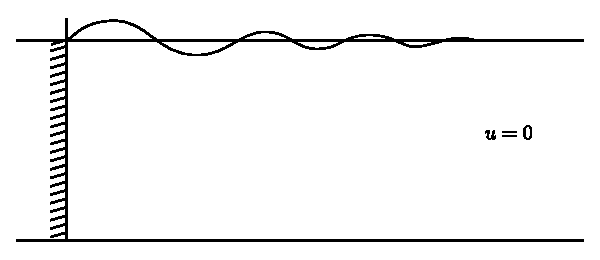
\includegraphics{figures/fig61-4.2.eps}
\caption{}
\label{chap1:fig4.2}
\end{figure}

The movement of the piston is represented in the $x,t$ plane by the curve
$$
x=X(t),\,u=\dot{X}(t),
$$
where $X(t)$ is a given function.
\begin{figure}[H]
\centering
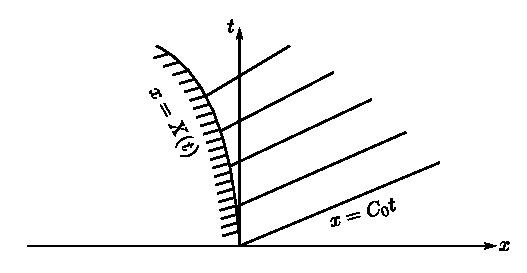
\includegraphics{figures/fig61-4.3.eps}
\caption{}
\label{chap1:fig4.3}
\end{figure}
\end{example*}

The\pageoriginale flow of water is governed by the equation 
$$
u_t+\left(c_0+\frac{3u}{2}\right)u_x=0,
$$
since a wave moving to the right is produced.

Following the constructions of chapter \ref{chap1}, we choose a characteristic curve on which 
$$
\frac{dx}{dt}=c_0+\frac{3u}{2}.
$$

On this characteristic $\frac{du}{dt}=0$; therefore, $u=\;\text{constant}\; = \dot{X}(\tau)$, if the characteristic is passing through $(X(\tau),\tau)$. Therefore, $\frac{dx}{dt}=c_0+\frac{3}{2}\dot{X} (\tau)$. 

Integrating we obtain
$$
x=X(\tau)+\left\{c_0+\frac{3}{2}\dot{X}(\tau)\right\}(t-\tau).
$$

Hence the solution of the piston problem is 
\begin{align*}
x &= X(\tau)+\left\{c_0+\frac{3}{2}\dot{X}(\tau)\right\}(t-\tau),\\
u &= \dot{X}(\tau),
\end{align*}
where $\tau$ is the characteristic parameter.

As in the previous cases, expansion waves (in this case $\ddot{X}(t)\leqq 0$) do not break and the solution is valid for all $t$. On the other hand, moving the piston forward or providing a positive acceleration, will produce a breaking wave. The inclusion of discontinuities based on the jump conditions (noted after equation \eqref{chap4:eq4.6}) is similar in spirit to the discussion of chapter \ref{chap3}, but is somewhat more complicated than before. The relation \eqref{chap4:eq4.10} is not strictly valid across discontinuities (note it was deduced from the differential\pageoriginale equations), and approximations have to be made if the simple wave solutions are still used. (See \cite{key1} for details in the equivalent gas dynamics case).

\section{Method of characteristics for a system}\label{chap4:sec4.3}

The above simple wave solutions provide an interesting approach and tie the discussion closely to the earlier material on a single equation. However, they are limited to waves moving in one direction only. We want to consider questions of waves moving in both directions and interacting with each other. We shall also find via Riemann's arguments a further understanding of the role of the simple waves.

Since we already know that $c=\sqrt{gh}$ is a useful quantity here, we shall introduce it at the outset to simplify the expressions but it is in no way crucial. The equations \eqref{chap4:eq4.7} and \eqref{chap4:eq4.8} then become
\begin{align}
u_t &+uu_x+2cc_x=0,\tag{4.13}\label{chap4:eq4.13}\\
c_t &+ uc_x+\frac{1}{2}\, cu_x=0.\tag{4.14}\label{chap4:eq4.14}
\end{align}

Now we note that each equation relates the directional derivatives of $u$ and $c$ for different directions. If the directions were the same we might make progress as in Chapter \ref{chap1}. But we can try linear combinations of \eqref{chap4:eq4.13} and \eqref{chap4:eq4.14} that have the desired property. Accordingly, we consider \eqref{chap4:eq4.13} $+m$. \eqref{chap4:eq4.14}, where $m$ is a quantity to be determined. We have 
\begin{equation}
\left\{u_t+uu_x+2cc_x\right\}+m\left\{c_t+uc_x+\frac{1}{2}\,cu_x\right\} =0\tag{4.15}\label{chap4:eq4.15}
\end{equation}\pageoriginale

This will take the desired form,
$$
\left\{u_t+vu_x\right\}+m\left\{c_t+vc_x\right\}=0,
$$
provided
$$
u+\frac{m}{2}c=u+\frac{2c}{m}=v.
$$

The latter gives $m=\pm 2$. Putting $m=2$ in \eqref{chap4:eq4.15} we have 
\begin{equation}
(u+2c)_t+(u+c)\;(u+2c)_x=0\tag{4.16}\label{chap4:eq4.16}
\end{equation}

We choose the $\mathscr{C}_+$ characteristic to be 
$$
\mathscr{C}_+:\frac{dx}{dt}=u+c
$$
On $\mathscr{C}_+$, \eqref{chap4:eq4.16} becomes, $\frac{d}{dt}(u+2c)=0$, which implies $u+2c=$ constant on $\mathscr{C}_+$.

Taking $m=-2$ in \eqref{chap4:eq4.15}, we obtain
\begin{equation}
(u-2c)_t+(u-c)\;(u-2c)_x=0\tag{4.17}\label{chap4:eq4.17}
\end{equation}
we choose the $\mathscr{C}_-$ characteristic with the property
$$
\mathscr{C}_-:\frac{dx}{dt}=u-c
$$
Then equation \eqref{chap4:eq4.17} implies: 
\begin{align*}
&\text{On}\quad \mathscr{C}_-,\frac{d}{dt}(u-2c)=0,\\
&\ie u-2c=\quad\text{constant on}\quad \mathscr{C}_-
\end{align*}

Thus we obtian
\begin{align*}
u+2c &= \quad\text{constant on}\quad \frac{dx}{dt}=u+c\\
u-2c &=\quad\text{constant on}\quad \frac{dx}{dt}=u-c
\end{align*}
The constants may differ from characteristic to characteristic.

This\pageoriginale is the method of characteristics for higher order systems. For an $n^{th}$ order system of first order equations for $u_1,\ldots,u_n$, one looks for a linear combination of the equations so that the directional derivatives of each $u_i$ is the same. If there are $n$ real different combinations with the characteristic property the system is {\bf hyperbolic}.

In the present case the characteristic equations will be useful in various ways. We first reconsider the simple wave solutions.

\section{Riemann's argument for simple waves}\label{chap4:sec4.4}

We focus on the piston problem to show how the argument goes through and refer to figure 4.4.
\begin{figure}[H]
\centering
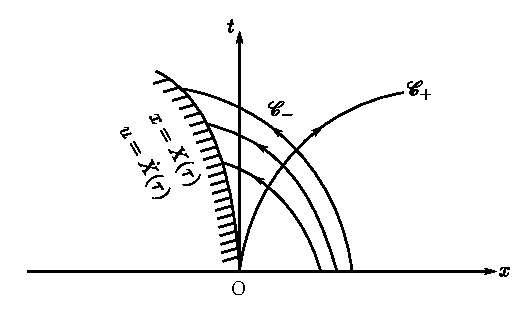
\includegraphics{figures/fig61-4.4.eps}
\caption{}
\label{chap1:fig4.4}
\end{figure}

Using the fact that $u-c\leqq u$ we can show that the $\mathscr{C}_-$ characteristics cover the whole region $\{(x,t):t\geqq 0,x\geqq X(t)\}$. On each $\mathscr{C}_-$ we have $u-2c=$ constant; from the initial condition 
$$
t=0:u=0,c=c_0,
$$
we find that $u-2c=-2c_0$. But\pageoriginale this is true for each $\mathscr{C}_-$ with the {\bf same} constant. Therefore 
\begin{equation}
u-2c=-2c_0\tag{4.18}\label{chap4:eq4.18}
\end{equation}
everywhere. This is exactly the relation \eqref{chap4:eq4.10}: We could now refer to the previous discussion to complete the solution. To complete the solution in the present context, we use the $\mathscr{C}_+$ relation
$$
u+2c=\quad\text{constant on}\quad\frac{dx}{dt}=u+c
$$
From \eqref{chap4:eq4.18} this becomes
$$
u=\quad\text{constant on}\quad\frac{dx}{dt}=c_o + \frac{3}{2}u, 
$$
exactly the information contained in \eqref{chap4:eq4.12}. We conclude that 
\begin{equation}
\left.
\begin{aligned}
u &= \dot{X}(\tau)\\
x &= X(\tau)+\left\{c_0+\frac{3}{2}\dot{X}(\tau)\right\}\;(t-\tau)
\end{aligned}
\right\}\tag{4.19}\label{chap4:eq4.19}
\end{equation}
as before.

\begin{problem*}
{\bf Dam break.} In an idealization, the flow of water out of a dam is governed by the equations
\begin{align*}
u_t &+ uu_x+2cc_x=0\\
c_t &+ uc_x+\frac{1}{2}\,cu_x=0
\end{align*}
with the initial conditions
\begin{equation*}
t=0:
\begin{cases}
u=0,\; -\infty < x < \infty,\\
h=
\begin{cases}
h_1,\; -\infty < x < 0,\\
0,\; 0< x < \infty.
\end{cases}
\end{cases}
\end{equation*}
\end{problem*}

Find the solution. (There is no discontinuity and the final answer takes a simple explicit form).

\section{Hodograph transformation}\label{chap4:sec4.5}\pageoriginale

In the interaction of waves, where both families of characteristics carry nontrivial disturbances (\ie \eqref{chap4:eq4.18} does not hold), solutions are much more difficult, and numerical methods are often used.

However, one alternative analytic method for studying the interaction of waves, or the two interacting families of waves produced by general initial conditions, is the `hodograph' method. The equations are 
\begin{equation}
\left.
\begin{aligned}
c_t +uc_x+\frac{1}{2}\,cu_x=0\\
u_t+uu_x+2cc_x=0
\end{aligned}
\right\}\tag{4.20}\label{chap4:eq4.20}
\end{equation}
and we note that the coefficients are functions of the dependent variables only. We try to make use of that fact by interchanging the role of dependent and independent variables.

We have $u=u(x,t),c=c(x,t)$ and consider the inverse functions 
$$
x=x(u,c),\;t=t(u,c).
$$

The term `hodograph' is used when the velocities $u$ and $c$ are considered as independent variables. We have the relations
\begin{align*}
c_t &= -\frac{x_u}{\mathfrak{g}}, c_x = \frac{t_u}{\mathfrak{g}},\\
u_t &=\frac{x_c}{\mathfrak{g}}, u_x= -\frac{t_c}{\mathfrak{g}},
\end{align*}
where $\mathfrak{g}=\frac{(c,t)}{(u,c)}=x_ut_c-x_ct_u$.

For the system \eqref{chap4:eq4.20}, the highly non-linear factor $\mathfrak{g}$ cancels through\pageoriginale and we have 
\begin{equation}
\left.
\begin{aligned}
x_u &=ut_u-\frac{1}{2}\,ct_c\\
x_c &=ut_c-2ct_u 
\end{aligned}
\right\}\tag*{$(4.20)'$}\label{chap4:eq4.20'}
\end{equation}

Notice $\mathfrak{g}$ would not cancel if there were undifferentiated
terms.\break Equations \ref{chap4:eq4.20'} are now linear and this offers
considerable simplification. 

Differentiating the first equation in \ref{chap4:eq4.20'} with respect to $c$, partially, and the second one with respect to $u$ and subtracting, we find 
\begin{equation}
4t_{uu}=t_{cc}+\frac{3}{c}t_c.\tag{4.21}\label{chap4:eq4.21}
\end{equation}

This is a linear equation for $t(u,c)$ which can be solved by standard methods.

However, the difficulties in this method are:
\begin{enumerate}
\item [(1)] The transformed boundary conditions in the $u-c$ plane will sometimes be awkward.
\item [(2)] When breaking occurs $\mathfrak{g}=0$, corresponding to the multivaluedness, and fitting in shocks may sometimes be difficult in this plane.
\end{enumerate}
For these reasons a numerical method is often preferred. However, in the case of waves on a sloping beach an analogous method has led to an extremely valuable solution; it will be described in section \ref{chap5:sec5.4}.

In that connection, a particularly elegant form of the transformation is useful and we note it here for the case of the horizontal bottom. We\pageoriginale use the characteristic form 
\begin{align*}
p &= u+2c =\quad\text{constant on}\quad\frac{dx}{dt}=u+c\\
q &=u-2c=\quad\text{constant on}\frac{dx}{dt}=u-c.
\end{align*}

If $p,q$ are used as variables, we can write
\begin{align*}
\frac{dx}{dt}&=u+c\\
\text{as}\qquad x_q &=(u+c)t_q,
\end{align*}
since $p$ is a constant on that characteristic and $q$ can be used as parameter. Similarly
$$
x_p=(u-c)t_p.
$$

We then substitute for $u$ and $c$ in terms of $p$ and $q$ to obtain
$$
x_q=\frac{3p+q}{4}t_q,\; x_p=\frac{p+3q}{4}t_p
$$
These are the linear hodograph equations equivalent to \ref{chap4:eq4.20'}. Eliminating $x$, we have 
$$
2(q-p)t_{pq}-3\left(t_q-t_p\right)=0,
$$
which is equivalent to \eqref{chap4:eq4.21}.





